\documentclass[11pt,letterpaper]{article}

\usepackage[margin=0.82in,headheight=22pt,footskip=26pt]{geometry}
\usepackage[T1]{fontenc}
\usepackage{newtxtext,newtxmath}
\usepackage{microtype}
\usepackage{amsmath,mathtools}
\usepackage{booktabs,tabularx,array}
\usepackage{enumitem}
\usepackage[dvipsnames]{xcolor}
\usepackage{tikz}
\usetikzlibrary{arrows.meta,positioning,calc}
\usepackage[most]{tcolorbox}
\usepackage{fancyhdr}
\usepackage{hyperref}
\usepackage{titlesec}
\usepackage{ragged2e}
\usepackage{caption}
\usepackage{float}
\usepackage{needspace}

\definecolor{navy}{HTML}{17365D}
\definecolor{teal}{HTML}{1D6F78}
\definecolor{pale}{HTML}{EEF4F7}
\definecolor{warm}{HTML}{F8F2E7}
\definecolor{rulegray}{HTML}{C8D0D8}
\definecolor{textgray}{HTML}{4D5966}
\definecolor{softgray}{HTML}{F5F6F7}
\definecolor{arrowgold}{HTML}{B67818}

\hypersetup{
  colorlinks=true,
  linkcolor=navy,
  urlcolor=teal,
  citecolor=navy,
  pdftitle={Modeling Pulsed NQR Dynamics: Spin 1, Spin 3/2, and Higher Spins},
  pdfsubject={Narrative modeling guidance for an NMR/NQR spin-dynamics package},
  pdfauthor={}
}

\pagestyle{fancy}
\fancyhf{}
\lhead{\small\color{textgray}Technical note: pulsed NQR modeling}
\rhead{\small\color{textgray}Spin 1, spin $3/2$, and higher spins}
\cfoot{\small\color{textgray}\thepage}
\renewcommand{\headrulewidth}{0.4pt}
\renewcommand{\headrule}{\hbox to\headwidth{\color{rulegray}\leaders\hrule height \headrulewidth\hfill}}

\titleformat{\section}{\Large\bfseries\color{navy}}{}{0pt}{}[\vspace{-2pt}\color{rulegray}\titlerule]
\titleformat{\subsection}{\large\bfseries\color{teal}}{}{0pt}{}
\titleformat{\subsubsection}{\normalsize\bfseries\color{navy}}{}{0pt}{}
\titlespacing*{\section}{0pt}{14pt}{7pt}
\titlespacing*{\subsection}{0pt}{10pt}{4pt}
\titlespacing*{\subsubsection}{0pt}{8pt}{3pt}

\setlength{\parindent}{0pt}
\setlength{\parskip}{5.4pt}
\setlist[itemize]{leftmargin=1.35em,itemsep=2.5pt,topsep=3pt}
\setlist[enumerate]{leftmargin=1.65em,itemsep=2.5pt,topsep=3pt}
\renewcommand{\arraystretch}{1.22}
\captionsetup{font=small,labelfont=bf,margin=10pt}

\newcommand{\HQ}{\hat H_Q}
\newcommand{\HZ}{\hat H_Z}
\newcommand{\Hrf}{\hat H_{\mathrm{rf}}}
\newcommand{\Tr}{\operatorname{Tr}}
\newcommand{\ket}[1]{\lvert #1\rangle}
\newcommand{\bra}[1]{\langle #1\rvert}
\newcommand{\dyad}[2]{\lvert #1\rangle\!\langle #2\rvert}

\newtcolorbox{openingbox}{
  colback=pale,colframe=teal,boxrule=0.75pt,arc=2pt,
  left=8pt,right=8pt,top=7pt,bottom=7pt
}
\newtcolorbox{scopebox}{
  colback=softgray,colframe=navy!60,boxrule=0.7pt,arc=2pt,
  left=8pt,right=8pt,top=7pt,bottom=7pt
}
\newtcolorbox{cautionbox}{
  colback=warm,colframe=arrowgold,boxrule=0.7pt,arc=2pt,
  left=8pt,right=8pt,top=7pt,bottom=7pt
}

\begin{document}

\begin{center}
{\LARGE\bfseries\color{navy}Modeling Pulsed NQR Dynamics}\\[4pt]
{\Large\color{teal}Why spin 1 can often be reduced to two levels, while spin $3/2$ and higher spins usually cannot}\\[8pt]
{\small Guidance for an NMR/NQR spin-dynamics simulation package}
\end{center}
\vspace{3pt}

\begin{openingbox}
\textbf{Purpose of this note.}
The package has to make a basic choice before it propagates a pulse sequence: should it retain every quantum level of the nucleus, or can it safely keep only the two levels belonging to one selected NQR transition? The answer is not determined by the number of peaks in a spectrum. It is determined by the number of states that the RF pulse can actually connect.

The current spin-1 implementation uses fictitious spin-$1/2$ operators for one selected transition. That is a useful and efficient model when the selected transition is isolated. The same idea is not a safe general default for spin $3/2$, because its apparently simple zero-field spectrum hides two degenerate pairs of states. The difference becomes especially important when a weak Zeeman field resolves those pairs.
\end{openingbox}

\section{What the simulator is trying to predict}

A pulsed NQR experiment applies one or more RF pulses and then detects the signal produced by the nuclear ensemble. The simulation must predict how the pulse redistributes \emph{population} among the energy levels and how it creates \emph{coherence} between them. Population determines how much of the ensemble occupies each level. Coherence carries the phase information that gives rise to an FID, an echo, or interference between different pulse pathways.

For a nucleus of spin $I$, the complete quantum state lives in a space of dimension
\begin{equation}
 d=2I+1.
\end{equation}
A \textbf{full model} retains all $d$ levels and propagates a $d\times d$ density matrix. The diagonal entries of that matrix are populations; the off-diagonal entries are coherences.

A \textbf{reduced two-level model} keeps only one selected pair of levels. The other levels still exist physically, but the calculation assumes that they do not participate. In this note, an omitted level is called a \textbf{spectator} when the pulse does not appreciably change its population and does not create appreciable coherence involving it. The word therefore describes a dynamical condition, not a new kind of state.

This distinction matters because a reduced model can reproduce the correct resonance frequency and still give the wrong pulse response. If an omitted level is weakly excited, the error may appear as a wrong nutation rate, echo amplitude, phase, orientation dependence, or response to a second pulse. The goal is not to avoid approximations; it is to make the approximation explicit and testable.

\section{The Hamiltonian: a map from the experiment to the levels}

In NQR, the electric-field gradient (EFG) at the nucleus supplies the dominant static interaction. In the principal-axis frame of the EFG tensor, a convenient convention-independent form is
\begin{equation}
\HQ=A\left[3I_{z'}^2-I(I+1)\mathbf 1
+\eta\left(I_{x'}^2-I_{y'}^2\right)\right],
\qquad 0\leq\eta\leq1,
\label{eq:HQ}
\end{equation}
where $A$ sets the quadrupole energy scale. The first part of Eq.~\eqref{eq:HQ} gives the axially symmetric level pattern. The asymmetry parameter $\eta$ measures how strongly the EFG distinguishes the $x'$ and $y'$ directions: $\eta=0$ is axial symmetry, while $\eta>0$ breaks that symmetry.

A static magnetic field and the RF pulse add
\begin{equation}
\HZ=-\hbar\gamma\,\mathbf B_0\!\cdot\!\mathbf I,
\qquad
\Hrf(t)=-\hbar\gamma\,\mathbf B_1(t)\!\cdot\!\mathbf I,
\qquad
\hat H(t)=\HQ+\HZ+\Hrf(t).
\label{eq:Htotal}
\end{equation}
The static Hamiltonian $H_0=H_Q+H_Z$ determines the energies and eigenstates before the pulse. The RF operator determines which pairs of those eigenstates are coupled by the coil polarization. Thus a simulator makes the modeling decision by examining two things together: the spacing of the transitions and the corresponding RF matrix elements.

The density matrix then evolves according to
\begin{equation}
\frac{d\rho}{dt}=-\frac{i}{\hbar}[H(t),\rho].
\label{eq:liouville}
\end{equation}
Equation~\eqref{eq:liouville} is the common starting point for every spin discussed below. The only question is how large a state space must be retained for it to describe the experiment honestly.

\section{Read the level structure before choosing a model}

Figure~\ref{fig:levelmap} shows the central distinction. Each horizontal line represents an energy level. Two lines drawn at the same height represent two different states with exactly the same energy. An arrow represents an RF-driven transition. The vertical spacing is schematic; the point of the figure is the number of states and the way the arrows connect them.

\begin{figure}[H]
\centering
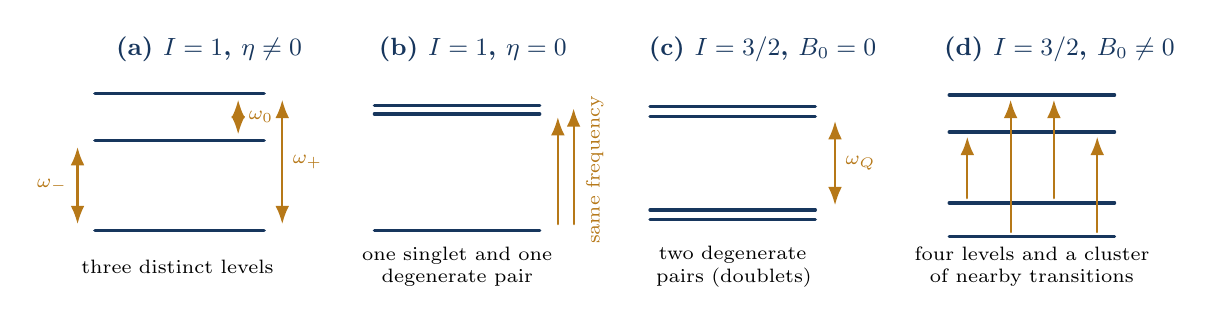
\begin{tikzpicture}[x=1cm,y=1cm,>=Latex,line cap=round,every node/.style={font=\small}]
  % panel a
  \node[font=\small\bfseries,text=navy] at (1.75,2.58) {(a) $I=1$, $\eta\neq0$};
  \draw[navy,very thick] (0.30,0.28)--(2.45,0.28);
  \draw[navy,very thick] (0.30,1.42)--(2.45,1.42);
  \draw[navy,very thick] (0.30,2.02)--(2.45,2.02);
  \draw[<->,arrowgold,thick] (0.08,0.36)--(0.08,1.34) node[midway,left,font=\scriptsize] {$\omega_-$};
  \draw[<->,arrowgold,thick] (2.68,0.36)--(2.68,1.94) node[midway,right,font=\scriptsize] {$\omega_+$};
  \draw[<->,arrowgold,thick] (2.12,1.50)--(2.12,1.94) node[midway,right,font=\scriptsize] {$\omega_0$};
  \node[font=\scriptsize,align=center,text width=3.1cm] at (1.35,-0.18) {three distinct levels};

  % panel b
  \node[font=\small\bfseries,text=navy] at (5.10,2.58) {(b) $I=1$, $\eta=0$};
  \draw[navy,very thick] (3.85,0.28)--(5.95,0.28);
  \draw[navy,very thick] (3.85,1.76)--(5.95,1.76);
  \draw[navy,very thick] (3.85,1.87)--(5.95,1.87);
  \draw[->,arrowgold,thick] (6.18,0.36)--(6.18,1.72);
  \draw[->,arrowgold,thick] (6.38,0.36)--(6.38,1.83);
  \node[font=\scriptsize,rotate=90,text=arrowgold] at (6.65,1.05) {same frequency};
  \node[font=\scriptsize,align=center,text width=3.1cm] at (4.90,-0.18) {one singlet and one degenerate pair};

  % panel c
  \node[font=\small\bfseries,text=navy] at (8.78,2.58) {(c) $I=3/2$, $B_0=0$};
  \draw[navy,very thick] (7.35,0.42)--(9.45,0.42);
  \draw[navy,very thick] (7.35,0.54)--(9.45,0.54);
  \draw[navy,very thick] (7.35,1.73)--(9.45,1.73);
  \draw[navy,very thick] (7.35,1.85)--(9.45,1.85);
  \draw[<->,arrowgold,thick] (9.70,0.60)--(9.70,1.67) node[midway,right,font=\scriptsize] {$\omega_Q$};
  \node[font=\scriptsize,align=center,text width=3.1cm] at (8.40,-0.18) {two degenerate pairs (doublets)};

  % panel d
  \node[font=\small\bfseries,text=navy] at (12.55,2.58) {(d) $I=3/2$, $B_0\neq0$};
  \draw[navy,very thick] (11.15,0.20)--(13.25,0.20);
  \draw[navy,very thick] (11.15,0.63)--(13.25,0.63);
  \draw[navy,very thick] (11.15,1.53)--(13.25,1.53);
  \draw[navy,very thick] (11.15,2.00)--(13.25,2.00);
  \draw[->,arrowgold,thick] (11.38,0.69)--(11.38,1.47);
  \draw[->,arrowgold,thick] (11.93,0.26)--(11.93,1.94);
  \draw[->,arrowgold,thick] (12.48,0.69)--(12.48,1.94);
  \draw[->,arrowgold,thick] (13.03,0.26)--(13.03,1.47);
  \node[font=\scriptsize,align=center,text width=3.3cm] at (12.20,-0.18) {four levels and a cluster of nearby transitions};
\end{tikzpicture}
\caption{The level structures that drive the modeling choice. In panel (a), finite asymmetry separates the three spin-1 levels. In panel (b), two spin-1 transitions collapse onto the same frequency. In panel (c), one spin-$3/2$ NQR frequency connects two degenerate pairs of states. A Zeeman field resolves those hidden states in panel (d). Arrows indicate possible RF pathways, not equal intensities.}
\label{fig:levelmap}
\end{figure}

Panel (a) is the situation in which a spin-1 reduction can work: a pulse may be tuned to one arrow while the third level is far enough away to remain inactive. Panel (b) shows why $\eta=0$ is different. The two arrows have the same frequency, so a generic RF pulse does not encounter a unique pair of levels.

Panel (c) looks spectrally simple because it contains only one energy difference. It is nevertheless a four-state system: both the lower and upper energies contain two states. Panel (d) makes that hidden structure visible. A weak magnetic field separates the states and turns the original line into several nearby components.

\section{Spin 1: a two-level model with a clear validity domain}

\subsection{Why finite asymmetry helps}

For $I=1$, convenient zero-field eigenstates are
\begin{equation}
\ket X=\frac{\ket{+1}+\ket{-1}}{\sqrt2},\qquad
\ket Y=\frac{\ket{+1}-\ket{-1}}{i\sqrt2},\qquad
\ket Z=\ket0.
\end{equation}
With the convention in Eq.~\eqref{eq:HQ}, their energies are
\begin{equation}
E_X=A(1+\eta),\qquad E_Y=A(1-\eta),\qquad E_Z=-2A,
\label{eq:spin1energies}
\end{equation}
and the three transition frequencies are
\begin{equation}
\omega_{XY}=\frac{2A\eta}{\hbar},\qquad
\omega_{XZ}=\frac{A(3+\eta)}{\hbar},\qquad
\omega_{YZ}=\frac{A(3-\eta)}{\hbar}.
\label{eq:spin1freq}
\end{equation}
These formulas explain the useful feature of asymmetric spin-1 NQR: when $\eta>0$, the three levels are no longer degenerate, and the three pairwise transition frequencies are generally distinguishable. Experiments that deliberately use all three frequencies demonstrate that all three levels are real dynamical participants; a single-transition model is a choice to work in a restricted regime, not a replacement for the three-level physics.\cite{sauer2001}

Suppose, for example, that the pulse is centered on the $Y\leftrightarrow Z$ transition. The reduced calculation keeps $\ket Y$ and $\ket Z$ and represents them as the ``up'' and ``down'' states of an effective spin $1/2$. The state $\ket X$ is the spectator only if the pulse is too far off resonance, or too weakly coupled by its polarization, to move population or coherence into that state.

\subsection{What fictitious spin-$1/2$ operators mean}

For any selected pair $\ket a,\ket b$, define
\begin{align}
X_{ab}&=\tfrac12(\dyad a b+\dyad b a),
&Y_{ab}&=\tfrac1{2i}(\dyad a b-\dyad b a),\\
Z_{ab}&=\tfrac12(\dyad a a-\dyad b b).
\end{align}
Within the selected pair these operators behave exactly like the usual Pauli operators. They are simply a convenient language for rotations and phase evolution on that transition.\cite{vega1978}

The operators themselves are not the approximation. The approximation is the decision not to propagate the matrix elements involving the third level. In a rotating frame, the selected pair then has the familiar form
\begin{equation}
\frac{H_{ab}^{\mathrm{eff}}}{\hbar}
\simeq \Delta\,Z_{ab}
+\Omega_1^{\mathrm{eff}}
\left(\cos\phi\,X_{ab}+\sin\phi\,Y_{ab}\right),
\end{equation}
where $\Delta$ is the detuning, $\Omega_1^{\mathrm{eff}}$ is the nutation rate on that particular transition, and $\phi$ is the RF phase.

\subsection{The practical test: can the pulse reach another transition?}

Let $t$ denote the transition being simulated, and define its distance from the nearest competing RF-active transition as
\begin{equation}
\Delta_{\mathrm{iso}}=\min_{j\neq t}|\omega_t-\omega_j|.
\label{eq:deltaiso}
\end{equation}
A useful design criterion is
\begin{equation}
\Delta_{\mathrm{iso}}\gg
\max\!\left(\Omega_1^{\mathrm{eff}},\,\Delta\omega_{\mathrm{pulse}},\,\Gamma\right).
\label{eq:isolation}
\end{equation}
The three quantities on the right describe three different ways in which the experiment can lose selectivity. A strong RF field power-broadens the response on the scale of $\Omega_1^{\mathrm{eff}}$. A short pulse has a broad frequency spectrum $\Delta\omega_{\mathrm{pulse}}$ (of order $1/t_p$ for a rectangular pulse). The sample itself contributes a linewidth or inhomogeneous spread $\Gamma$. If any of these scales approaches the spacing to another active transition, the third level is no longer safely ignored.

The symbol ``$\gg$'' is deliberately a modeling criterion rather than a universal numerical threshold. A package can choose a conservative ratio and should validate it against the full $3\times3$ calculation over representative pulse powers, offsets, and orientations.

\begin{cautionbox}
\textbf{Why $\eta\neq0$ is necessary but not sufficient.}
At $\eta=0$, Eq.~\eqref{eq:spin1energies} gives $E_X=E_Y$, and the two finite-frequency transitions $X\leftrightarrow Z$ and $Y\leftrightarrow Z$ coincide. A generic pulse therefore addresses a one-to-two connection rather than a unique two-state pair. A special single-crystal polarization can sometimes select a bright combination and leave an orthogonal dark combination, but that is an additional symmetry assumption. It should not be the default meaning of the current spin-1 module.

For small nonzero $\eta$, the transitions may still be unresolved. Equation~\eqref{eq:isolation}, not the logical test $\eta\neq0$ by itself, is the operative validity check.
\end{cautionbox}

\begin{scopebox}
\textbf{Recommended scope statement for the current spin-1 implementation.}
The spin-1 NQR module uses fictitious spin-$1/2$ operators for one selected quadrupolar transition. This is a reduced, transition-selective model. It requires a nonzero EFG asymmetry parameter and, more importantly, a selected transition that is isolated on the scale of the RF nutation rate, pulse bandwidth, and linewidth. At $\eta=0$, or whenever a pulse addresses more than one transition or transfers coherence through the third level, the package should use a full $3\times3$ spin-1 density matrix or a separately documented symmetry-adapted model.
\end{scopebox}

\section{Spin $3/2$: why one NQR line can still require four states}

\subsection{The degeneracy is the essential difference}

A half-integer spin at zero magnetic field obeys a time-reversal symmetry that forces every energy to occur at least twice. The resulting equal-energy pair is called a \textbf{Kramers doublet}. This is not a small-splitting approximation: at $B_0=0$ the degeneracy is exact as long as the Hamiltonian is time-reversal invariant.

For $I=3/2$, the quadrupole Hamiltonian has only two distinct energies,
\begin{equation}
E_{\pm}=\pm A\sqrt{9+3\eta^2},
\label{eq:spin32energy}
\end{equation}
with each energy occurring twice. EFG asymmetry changes the energy separation and mixes the basis states, but it cannot split either doublet. The zero-field spectrum therefore contains one principal NQR frequency,
\begin{equation}
\omega_Q=\frac{E_+-E_-}{\hbar},
\end{equation}
while the quantum system still contains four states.

This is the point that a line-counting argument misses. ``One line'' means one energy difference. It does not mean that only one lower state and one upper state exist.

\subsection{What the Zeeman perturbation changes}

Adding $H_Z=-\hbar\gamma\mathbf B_0\cdot\mathbf I$ breaks time-reversal symmetry and lifts the degeneracy. Each doublet separates into two levels. If the field is not aligned with an EFG principal axis, it also changes the eigenvectors rather than merely shifting their energies. The RF operator, expressed in that new eigenbasis, can then contain several nonzero matrix elements between the lower and upper levels. Zeeman-perturbed spin-$3/2$ NQR experiments are consequently sensitive to the field magnitude, field direction, RF polarization, and the phases accumulated on several nearby pathways.\cite{panguluri2006,teles2015}

A pulse whose bandwidth covers more than one of those components acts on a connected four-state system. Treating the components as unrelated spin-$1/2$ transitions can lose three kinds of information:
\begin{itemize}
\item population deposited in a state by one pathway can change what another pathway can do;
\item coherences on different pathways acquire relative phases and may interfere in an echo;
\item an oblique Zeeman field can mix the states, so the transition strengths themselves change with orientation.
\end{itemize}
These are not higher-order details if the pulse actually covers the split line cluster. They are the pulse dynamics the simulation is intended to predict.

\subsection{The straightforward model is the complete $4\times4$ density matrix}

Construct the usual spin-$3/2$ matrices, form
\begin{equation}
H_0=H_Q+H_Z,
\end{equation}
and diagonalize $H_0$ for the actual EFG and field orientation. The eigenvalue differences give the transition frequencies. The transformed matrix elements of $\hat{\mathbf e}_1\cdot\mathbf I$ give the RF couplings for the coil polarization $\hat{\mathbf e}_1$.

For a pulse or free-evolution interval during which the Hamiltonian is constant, the propagation is
\begin{equation}
U_k=\exp\!\left(-\frac{i}{\hbar}H_k\Delta t_k\right),
\qquad
\rho_{k+1}=U_k\rho_kU_k^{\dagger}.
\label{eq:propagate}
\end{equation}
The first equation says how the four-state system evolves during one time segment. The second applies that evolution to both populations and coherences. A shaped pulse is handled by dividing it into short segments and repeating the same update. The detected signal is then
\begin{equation}
s(t)=\Tr\!\left[\rho(t)M_{\mathrm{det}}\right],
\end{equation}
where $M_{\mathrm{det}}$ represents the receive-coil observable.

This is numerically modest: the state is only a $4\times4$ matrix. If relaxation is needed, the same problem can be written in a $16$-dimensional Liouville space, where populations and different coherence modes can be assigned appropriate relaxation behavior.\cite{harel2006,odin2017}

A two-level spin-$3/2$ reduction is still possible in a deliberately restricted experiment--for example, when one Zeeman-resolved transition is much farther from its neighbors than the pulse bandwidth and the RF polarization suppresses the other branches. The important policy is that such a reduction is a named, verified special case. It is not the default representation of Zeeman-perturbed spin-$3/2$ NQR.

\section{Spins greater than $3/2$: more levels, and new ways to couple them}

The equation of motion does not change for higher spin. What changes is the size and connectivity of the level system. A spin-$5/2$ nucleus has six states, a spin-$7/2$ nucleus has eight, and so on. Two broad families need to be distinguished.

\subsection{Half-integer spins: ladders of Kramers doublets}

Every half-integer spin retains Kramers degeneracy at zero field. Spin $5/2$ has three doublets; spin $7/2$ has four; spin $9/2$ has five. In an axial EFG, the main NQR frequencies connect neighboring doublets. Thus an isolated spectral line naturally involves the two doublets on either side of that frequency--up to four states--even before adjacent NQR lines are considered. Special symmetry and polarization can divide this four-state space into smaller independent blocks, but the simulator should establish that from the matrix elements rather than assume it.

Higher half-integer spins also have neighboring NQR lines that share a doublet. For spin $5/2$, for example, the lower-frequency transition and the higher-frequency transition both involve the middle doublet. If a broadband pulse reaches both lines, the two excitations are not two independent spin-$1/2$ experiments. Population or coherence placed in the shared doublet by one line immediately affects the other. Exact density-matrix treatments of spin $5/2$, spin $7/2$, and general time-domain NQR make this connected structure explicit.\cite{nagel1995,ageev1996,harel2006}

\subsection{Integer spins: asymmetry may split levels, but not always by a useful amount}

Integer spins are not protected by Kramers' theorem. In an asymmetric EFG their levels can, in principle, become nondegenerate singlets. The spin-1 lesson nevertheless does not generalize as the simple rule ``$\eta\neq0$ implies isolated transitions.''

Near axial symmetry, the states $\ket{+m}$ and $\ket{-m}$ begin as degenerate pairs. The asymmetry operator can be written as
\begin{equation}
I_{x'}^2-I_{y'}^2=\tfrac12\left(I_+^2+I_-^2\right),
\label{eq:dm2}
\end{equation}
so one application changes $m$ by two units. For spin 2, the states $\ket{+1}$ and $\ket{-1}$ are coupled directly and their splitting begins at first order in $\eta$. The states $\ket{+2}$ and $\ket{-2}$ communicate only through $\ket0$, so their splitting begins at second order. More generally, high-$|m|$ pairs can remain extremely close even though $\eta$ is formally nonzero. The package must therefore inspect the actual eigenvalue differences rather than infer spectral resolution from $\eta$ alone.

\subsection{Effects that become increasingly important}

\textbf{A single pulse angle is no longer universal.}
Even in the axial basis, the coupling strength of an adjacent transition is
\begin{equation}
\left|\bra{m-1}I_x\ket m\right|
=\frac12\sqrt{I(I+1)-m(m-1)}.
\label{eq:matrixelement}
\end{equation}
The same RF amplitude therefore produces different nutation rates on different transitions. A pulse calibrated as a $90^\circ$ pulse on one line is generally not a $90^\circ$ pulse on another. At finite $\eta$, Eq.~\eqref{eq:matrixelement} is replaced by the corresponding matrix element between the exact mixed eigenstates, but the physical conclusion is unchanged.

\textbf{Strong or broadband pulses can create multiple-quantum coherence.}
The static asymmetry mixes bare $m$ states, and a finite-duration pulse can link several parts of the level network. Coherences may then appear between states separated by more than one nominal $m$ step. These pathways can generate additional echoes or phase dependences. They are physical consequences of the multilevel system, not numerical artifacts.

\textbf{Intermediate magnetic fields can reorganize the spectrum.}
When the Zeeman and quadrupole energies are comparable, eigenstates can exchange character near avoided crossings. Transition intensity can move rapidly from one line to another as field magnitude or orientation changes. Direct diagonalization of $H_Q+H_Z$ follows this evolution continuously; a collection of hand-selected two-level formulas does not.

\textbf{Relaxation has more modes.}
A higher-spin density matrix contains several independent population differences and many coherence orders. One pair of Bloch constants, $T_1$ and $T_2$, may be adequate for a qualitative model but is not a general description. A $d^2$-dimensional Liouville-space model is the natural extension when quantitative relaxation is required.

\begin{table}[H]
\centering
\small
\begin{tabularx}{\textwidth}{>{\RaggedRight\arraybackslash\bfseries}p{0.13\textwidth}>{\RaggedRight\arraybackslash}p{0.13\textwidth}>{\RaggedRight\arraybackslash}X>{\RaggedRight\arraybackslash}X}
\toprule
Spin & Full dimension & Zero-field structure & Sensible default \\
\midrule
$1$ & $3\times3$ & Three singlets for generic $\eta>0$; a degenerate pair at $\eta=0$ & Use the selected two-level path only after the isolation test; keep a full $3\times3$ reference path. \\
$3/2$ & $4\times4$ & Two Kramers doublets for every $\eta$ & Full four-state propagation, especially with Zeeman perturbation. \\
$2$ & $5\times5$ & Axial $\pm m$ pairs can split into singlets, sometimes only weakly & Full five-state propagation unless an actual transition analysis proves a smaller active block. \\
$5/2$ & $6\times6$ & Three Kramers doublets & Full six-state propagation when more than one line is excited; an isolated line still naturally spans two doublets. \\
$7/2$ & $8\times8$ & Four Kramers doublets & Full eight-state propagation is inexpensive and avoids hand-built pathway assumptions. \\
\bottomrule
\end{tabularx}
\caption{The matrix dimension grows slowly for a single nucleus. The difficult part is usually orientation averaging and waveform sampling, not the dense linear algebra of a $d\times d$ matrix.}
\end{table}

\section{Recommended package architecture}

A single full-spin backend can support every case. For a requested spin $I$, construct $I_x$, $I_y$, and $I_z$ in the Zeeman basis; form $H_Q+H_Z$; diagonalize it for the current orientation; transform the RF and detection operators into that eigenbasis; and propagate the $d\times d$ density matrix through the pulse sequence.

The existing spin-1 fictitious-spin path can remain as an optimized front end. It should call a model-selection check rather than being selected from $I=1$ alone. A practical sequence is:
\begin{enumerate}
\item Compute the eigenvalues and eigenvectors of the actual static Hamiltonian.
\item Build the transition catalogue from the RF matrix elements for the actual coil polarization.
\item Identify which transitions lie within the pulse spectrum and which states those transitions connect.
\item Use the two-level path only when the pulse-addressed connected set contains one pair of states and leakage to every excluded state is below the chosen tolerance.
\item Otherwise use the full active block or, for these small single-spin systems, the complete $(2I+1)$-level model.
\end{enumerate}

This organization keeps the approximation where it belongs: in a transparent model-selection layer. The propagation engine itself remains generic.

The most useful diagnostics are also physical ones. When the package chooses a reduced model, it should report the selected states, the target transition, the nearest competing RF-active transition, the estimated pulse bandwidth, and the isolation ratio. For spin 1 it should warn or fall back at $\eta=0$. For spin $3/2$ and higher half-integer spins it should make clear when a degenerate doublet has been split or projected by an additional assumption.

\section{Conclusion}

The difference between spin 1 and spin $3/2$ is not simply that one has three levels and the other has four. The important difference is how those levels are grouped by symmetry and how an RF pulse connects them.

For spin 1 with finite asymmetry, the three states can be spectrally distinct. A pulse placed on one isolated transition can then act on a closed pair while the third level remains a spectator. This is the regime in which the current fictitious-spin-$1/2$ implementation is both useful and honest. The documentation should say explicitly that $\eta\neq0$ is required but not sufficient; the real condition is transition isolation on the scale of pulse bandwidth, nutation rate, and linewidth.

For spin $3/2$, the zero-field quadrupole spectrum consists of two Kramers doublets. One observed NQR frequency therefore hides four states. A Zeeman field reveals that structure by splitting and mixing the doublets, and a realistic pulse can drive several nearby pathways at once. The straightforward general model is the full $4\times4$ density matrix.

For spins above $3/2$, the same full-space method continues to work. Half-integer spins add more Kramers doublets and shared transition ladders. Integer spins can split into singlets, but some near-axial splittings may remain too small to resolve. Transition-specific nutation rates, multiple-quantum pathways, intermediate-field mixing, and richer relaxation all make model selection more dependent on the actual Hamiltonian and pulse. A generic $(2I+1)$-level backend, with carefully validated reductions as optional optimizations, is therefore the simplest architecture that remains physically transparent.

\Needspace{8\baselineskip}
\begin{thebibliography}{9}
\small
\bibitem{das1958}
T. P. Das and E. L. Hahn, \textit{Nuclear Quadrupole Resonance Spectroscopy}, Solid State Physics Supplement 1, Academic Press (1958).

\bibitem{sauer2001}
K. L. Sauer, B. H. Suits, A. N. Garroway, and J. B. Miller, ``Three-frequency nuclear quadrupole resonance of spin-1 nuclei,'' \textit{Chemical Physics Letters} \textbf{342}, 362--368 (2001). \href{https://doi.org/10.1016/S0009-2614(01)00602-9}{doi:10.1016/S0009-2614(01)00602-9}.

\bibitem{vega1978}
S. Vega, ``Fictitious spin-$1/2$ operator formalism for multiple quantum NMR,'' \textit{Journal of Chemical Physics} \textbf{68}, 5518--5527 (1978). \href{https://doi.org/10.1063/1.435679}{doi:10.1063/1.435679}.

\bibitem{panguluri2006}
R. P. Panguluri and B. H. Suits, ``Spin $3/2$ Zeeman perturbed NQR in the presence of slow sample rotation,'' \textit{Journal of Magnetic Resonance} \textbf{182}, 49--54 (2006). \href{https://doi.org/10.1016/j.jmr.2006.06.008}{doi:10.1016/j.jmr.2006.06.008}.

\bibitem{harel2006}
E. Harel and H. Cho, ``A general numerical analysis of time-domain NQR experiments,'' \textit{Journal of Magnetic Resonance} \textbf{183}, 308--314 (2006). \href{https://doi.org/10.1016/j.jmr.2006.06.033}{doi:10.1016/j.jmr.2006.06.033}.

\bibitem{odin2017}
C. Odin, ``Repetitive experiments of one or two-pulse sequences in NQR of spins $I=3/2$: Liouville space, steady-state, Ernst angle and optimum signal,'' \textit{Solid State Nuclear Magnetic Resonance} \textbf{85--86}, 25--33 (2017). \href{https://doi.org/10.1016/j.ssnmr.2017.04.004}{doi:10.1016/j.ssnmr.2017.04.004}.

\bibitem{teles2015}
J. Teles, C. Rivera-Ascona, R. S. Polli, R. Oliveira-Silva, E. L. G. Vidoto, J. P. Andreeta, and T. J. Bonagamba, ``Experimental implementation of quantum information processing by Zeeman-perturbed nuclear quadrupole resonance,'' \textit{Quantum Information Processing} \textbf{14}, 1889--1906 (2015). \href{https://doi.org/10.1007/s11128-015-0967-3}{doi:10.1007/s11128-015-0967-3}.

\bibitem{nagel1995}
O. A. Nagel et al., ``Density matrix calculation of spin $5/2$ pure nuclear quadrupole resonance echoes,'' \textit{Physica A} \textbf{218}, 487--506 (1995). \href{https://doi.org/10.1016/0378-4371(95)00158-4}{doi:10.1016/0378-4371(95)00158-4}.

\bibitem{ageev1996}
S. Z. Ageev and B. C. Sanctuary, ``Selective excitation of single and multiple quantum transitions for spin $7/2$ in NQR,'' \textit{Molecular Physics} \textbf{87}, 1423--1438 (1996). \href{https://doi.org/10.1080/00268979600100961}{doi:10.1080/00268979600100961}.
\end{thebibliography}

\end{document}
